\RequirePackage{luatex85}
\documentclass[tikz, border=10pt]{standalone}

\usepackage[compat=1.1.0]{tikz-feynman}

\begin{document}

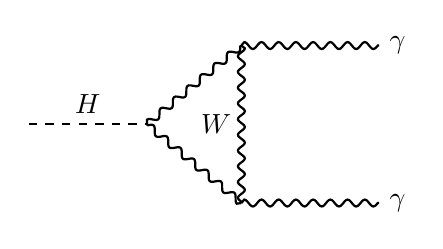
\begin{tikzpicture}[thick]
 \begin{feynman}
  \vertex (origin);
  \vertex [right=1.5cm of origin] (H);
  \vertex [above right=1cm and 1.2cm of H] (v1);
  \vertex [below right=1cm and 1.2cm of H] (v2);
  \vertex [right=1.75cm of v1] (gamma1) {\(\gamma\)};
  \vertex [right=1.75cm of v2] (gamma2) {\(\gamma\)};
  \diagram* {
  (origin) -- [scalar, edge label={\(H\)}] (H),
  (H) -- [boson] (v2) -- [boson, edge label={\(W\)}] (v1) -- [boson] (H),
  (gamma1) -- [photon] (v1),
  (gamma2) -- [photon] (v2),
  };
 \end{feynman}
\end{tikzpicture}
\end{document}
